\chapter{Классификация существующих решений}

    \section{Существующие решения}

        Задача достижения консенсуса берет свое начало с публикации в 1982 году Лесли Лэмпортом, Робертом Шостаком и Маршалом Пизосом задачи о Византийских генералах\cite{lamportbft}. В данной задаче рассматривается алгоритм принятия согласованного решения группой турецких генералов путем обмена сообщениями.

        На текущий момент разработано множество алгоритмов консенсуса, каждый из которых решает собственный подкласс задач.
        
        Одним из видов классификации алгоритмов консенсуса является классификация по принципу принятия решения \cite{nguyen2018survey}: 
        
        \begin{itemize}
            \item алгоритмы основанные на голосовании
            \item алгоритмы основанные на доказательстве
        \end{itemize}

        \subsection{Алгоритмы, основанные на голосовании}

            Общей чертой алгоритмов, основанных на голосовании является выдвижение нового значения одним из участников и последующее голосование за принятия данного значения. Если определенная доля участников голосуют за новое значение, то оно считается принятым

            \subsubsection{Паксос}
            
                Паксос\cite{lamport2001paxos} --- алгоритм консенсуса, предназначенный для согласования одного единственного значения группой участников. Данный алгоритм является эксклюзивным, устойчивым к падению.
                
                Алгоритм Паксос определяет 3 роли для процессов участников:
                
                \begin{enumerate}
                    \item Заявитель
                    \item Избиратель
                    \item Ученик
                \end{enumerate}
                
                Каждый из узлов может принимать несколько из ролей одновременно. Заявитель получается новое значение от клиента, выдвигает его избирателям и предлагает проголосовать за него. Избиратель ответственен за голосование по предложению заявителя. Ученик информируется о результатах голосования, но не принимает в нем участия.
                
                Выполнение алгоритма разделяется на 2 этапа: подготовка и принятия. Пример работы алгоритма представлен на рисунке \ref{fig:paxos}.
                
                \begin{figure}
                    \centering
                    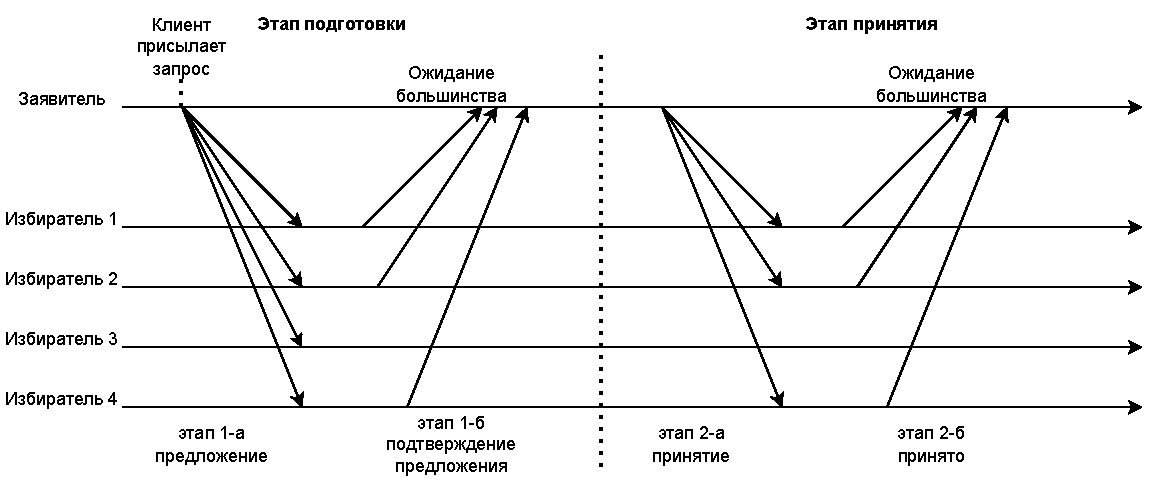
\includegraphics[width=\textwidth,height=25cm,keepaspectratio]{inc/img/paxos.pdf}
                    \caption{Пример работы алгоритма Паксос} \label{fig:paxos}
                \end{figure}
                
                \paragraph{Этапы выполнения:}
                
                    \begin{enumerate}
                        \item Подготовка. На данном этапе заявитель рассылает избирателям сообщения с номером раунда и новым значения для голосования. Избиратели голосуют, готовы ли они принять данное значение. Этап подготовки необходим для определения, является ли текущее предложение актуальным. Актуальность предложения определяется по номеру раунда. Избиратели сохраняют последний номер раунда, за который они голосовали. Если в предложении номер раунда выше, чем сохраненный номер, то предложение считается актуальным и избиратель сообщает заявителю о свой готовности на него проголосовать.
                        \item Принятие. На данном этапе заявитель определяет сколько избирателей готовы проголосовать за новое значение. Если готовы проголосовать более половины избирателей, то рассылается сообщение о фиксации данного значения и значение считается принятым системой.
                    \end{enumerate}
                
            \subsubsection{Рафт}
            
                Рафт\cite{ongaro2014search} --- алгоритм консенсуса, предназначенный для решения задачи репликации журнала. Данный алгоритм является эксклюзивным, устойчивым к падению.
                
                Алгоритм Рафт основывается на идеях алгоритма Паксос, но решает проблему его низкой производительности. Так в алгоритме Паксос для определения каждым узлом актуального значения необходимо обменяется \( n^2 \) сообщениями, где \( n \) --- число узлов в сети, так как каждый узел должен опросить все остальные узлу о принятом ими значении. Рафт решает данную проблему введением явного лидера, ответственного за информирование участников об актуальном состоянии принятого значения.
                
                Алгоритм Рафт определяет 3 роли:
                
                \begin{enumerate}
                    \item Лидер
                    \item Последователь
                    \item Кандидат
                \end{enumerate}
                
                Во всей системе может быть только один лидер, он ответственен за получение сообщений от клиента, управление журналом и общение с последователями. Последователь ответственен за сохранение записей журнала, получаемых от лидера. Кандидатом становится последователь, в случае долгого не получения сообщений от лидера. Кандидат выдвигает свою кандидатуру в качестве лидера и проводит голосование. Диаграмма переходов ролей представлена на рисунке \ref{fig:raft}.
                
                \begin{figure}
                    \centering
                    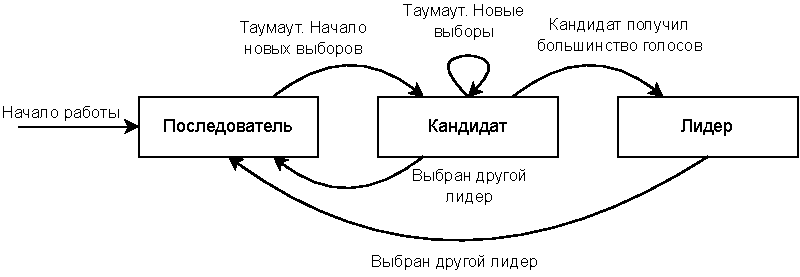
\includegraphics[width=\textwidth,height=25cm,keepaspectratio]{inc/img/raft.pdf}
                    \caption{Диаграмма переходов ролей в алгоритме Рафт} \label{fig:raft}
                \end{figure}

                Алгоритм Рафт вводит понятие эры. Эра --- период работы лидера. Концом и началом каждой эры является выбор нового кандидата в качестве лидера.

            \subsubsection{pBFT}

                pBFT\cite{castro1999practical} --- алгоритм консенсуса, предназначенный для согласования единственного значения в сети, где возможно византийское поведение участников. Данный алгоритм является инклюзивным.
                
                Данный алгоритм определяет 2 роли:
                
                \begin{enumerate}
                    \item Основной узел
                    \item Копия
                \end{enumerate}
                
                Основной узел инициирует начало работы алгоритма, в дальнейшем обменимавается сообщениями с копиями на равных условиях.
                
                pBFT определяет 3 этапа: предподготовка, подготовка, фиксация. Пример работы алгоритм представлен на рисунке \ref{fig:pbft}.
                
                \begin{figure}
                    \centering
                    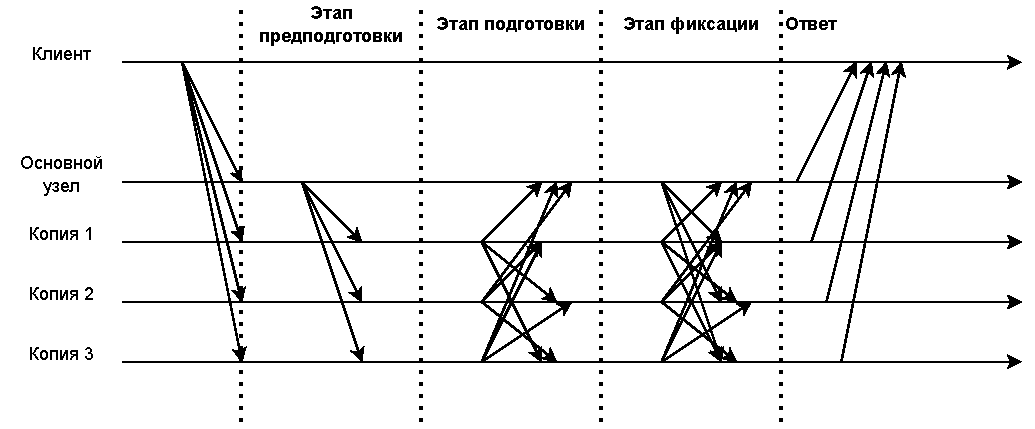
\includegraphics[width=\textwidth,height=25cm,keepaspectratio]{inc/img/BFT.pdf}
                    \caption{Пример работы алгоритма pBFT} \label{fig:pbft}
                \end{figure}

                
                \paragraph{Этапы выполнения:}
                
                    \begin{enumerate}
                        \item В самом начале клиент рассылает сообщение на все узлы системы.
                        \item Предподготовка. На данном этапе основной узел рассылает следующие сообщения на копии \textit{<PRE-PREPARE, H(m), s, v>}, где \textit{H(m)} --- хэш-сумма сообщения клиента, \textit{s} --- номер сообщения, \textit{v} --- последовательный номер основного узла. Данное сообщение подписывается электронном подписью перед отправкой.
                        \item Подготовка. При получении копией сообщения, копия проверяет электронную подпись, хэш-сумму сообщения и номер основного узла. В случае успешной проверки копия посылает следующее сообщения на все узлы сети: \textit{<PREPARE, H(m), s, v>}, где \textit{H(m)}
                        \item Фиксация. Если узел получил \( f \) некорректных сообщений и не меньше чем \( 2f + 1 \) корректных сообщений, то копия устанавливает значение и отправляет подтверждение клиенту. Значение считается установленным.
                    \end{enumerate}
                
                Алгоритм pBFT корректно работает в случае \( n >= 3f + 1 \), где \( n \) --- число честных узлов, \( f \) --- число византийских узлов.

        \subsection{Алгоритмы, основанные на доказательстве}

            Алгоритмы, основанные на доказательстве, предназначены для работы в сетях с неограниченным количеством узлов, поэтому в них не может быть применено голосование, так как злоумышленник может владеть неограниченным количеством узлов. Альтернативой подходу голосования является доказательство узлам сети своего более квалифицированного права на фиксацию значения.

            \subsubsection{Доказательство выполнения работы}

                Доказательство выполнения работы\cite{gervais2016security} --- алгоритм консенсуса, применяемый в блокчейн проектах, требующий от участников сети решение сложного криптографического пазла. Решение пазла не может быть предсказано заранее и требует от узла долгих вычислений. Блок узла, первого решившего задачу, добавляется в блокчейн. Примером такой задачи является генерация от блока хэш-суммы, меньшей заданного значения. Схема работы алгоритма представлена на рисунке \ref{fig:pow}
                
                Данный алгоритм считается устойчивым к византийскому поведению. Он сохраняет свою работоспособность, если злоумышленник владеет не больше чем \( 50\% \) вычислительных мощностей.
                
                \begin{figure}
                    \centering
                    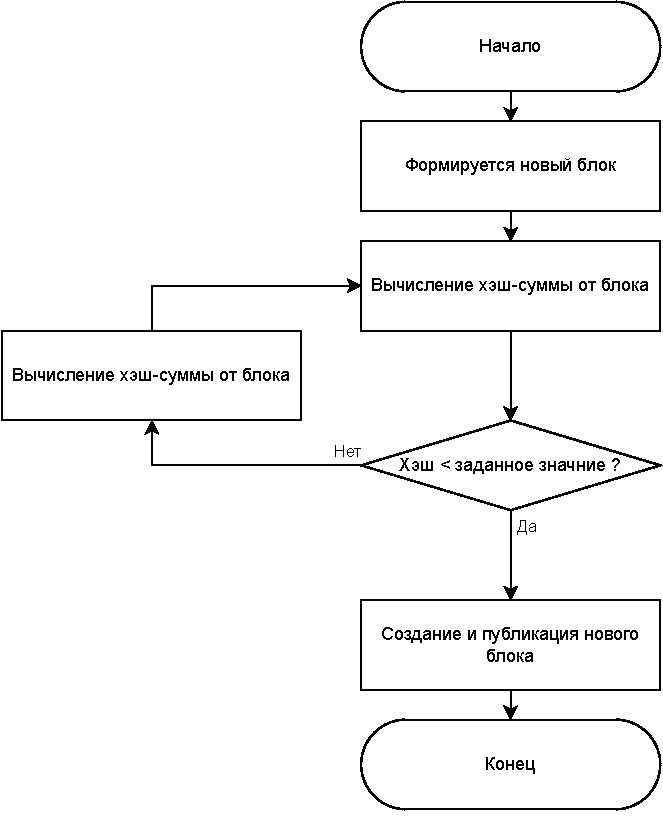
\includegraphics[width=\textwidth/2,height=15cm,keepaspectratio]{inc/img/pow.pdf}
                    \caption{Схема алгоритма доказательства выполнения работы} \label{fig:pow}
                \end{figure}

            \subsubsection{Доказательство доли владения}

                Доказательство доли владения\cite{king2012ppcoin} --- еще алгоритм консенсуса, применяемый в блокчейн проектах. Данный алгоритм является альтернативой алгоритму доказательству выполнения работы и решает проблему больших вычислительных затрат для добавления нового блока в блокчейн.
                
                При использовании этого метода алгоритм формирования блока не зависит от мощности оборудования, но с большей вероятностью блок будет сформирован той учетной записью, у которой текущий баланс больше. Например, участник, владеющий \( 1\%  \) от суммарного количества, в среднем будет генерировать \( 1\% \) новых блоков.
    
    \section{Критерии оценивания}
    
        \subsection{Классификация по модели принятия решения}
        
            По модели принятия решений алгоритмы консенсуса делятся на 2 типа:
            
            \begin{enumerate}
                \item Алгоритмы, основанные на голосовании
                \item Алгоритмы, основанные на доказательстве
            \end{enumerate}
            
            Общей чертой алгоритмов, основанных на голосовании, является выдвижение нового значения и голосовании на него участниками системы. Значение считается принятым, если за него проголосовали больше половины участников. Такие алгоритмы применяется в эксклюзивных сетях, где устанавливается количество участников, что позволяется определить отношение количества проголосовавших участников ко всем участникам.
            
            В алгоритмах, основанных на доказательстве, чаще применяются в инклюзивных блокчейнах. Участники системы соревнуются между собой за право создать новый блок.
            
            Классификация алгоритмов по данному критерию представлена в таблице \ref{tbl:classif_method}.
            
\begin{table}[h!]
	\begin{center}
		\caption{Классификация алгоритмов консенсуса по методу принятия решения}
		\label{tbl:classif_method}
		\begin{tabular}{|c|c|}
		\hline
		\textbf{Алгоритм} & \textbf{Тип} \\
		\hline
		Паксос & Основанный на голосовании \\
		\hline
		Рафт & Основанный на голосовании \\
		\hline
		pBFT & Основанный на голосовании \\
		\hline
		Доказательство выполнения работы & Основанный на доказательстве \\
		\hline
		Доказательство доли владения & Основанный на доказательстве \\
		\hline
        \end{tabular}
	\end{center}        
\end{table}

        \subsection{Классификация по эксклюзивности}

            По типу эксклюзивности алгоритмы консенсуса делятся на 2 типа:
            
            \begin{enumerate}
                \item Экслюзивные
                \item Инклюзивные
            \end{enumerate}
            
            В эксклюзивных алгоритмах достижения консенсуса принимать участие в работе алгоритма могут только заранее установленные узлы в ограниченном количестве. В инклюзивных алгоритмах такое ограничение снимается, принимать участие в них может любой желающий узел
            
            Классификация алгоритмов по данному критерию представлена в таблице \ref{tbl:classif_inclusive}.
        
\begin{table}[h!]
	\begin{center}
		\caption{Классификация алгоритмов консенсуса по эксклюзивности}
		\label{tbl:classif_inclusive}
		\begin{tabular}{|c|c|}
		\hline
		\textbf{Алгоритм} & \textbf{Тип} \\
		\hline
		Паксос & Эксклюзивный \\
		\hline
		Рафт & Эксклюзивный \\
		\hline
		pBFT & Эксклюзивный \\
		\hline
		Доказательство выполнения работы & Инклюзивный \\
		\hline
		Доказательство доли владения & Инклюзивный \\
		\hline
        \end{tabular}
	\end{center}        
\end{table}
        
        \subsection{Классификация по типу отказоустойчивости}

            По типу отказоустойчивости алгоритмы консенсуса делятся на 2 типа:
            
            \begin{enumerate}
                \item Устойчивость к падению
                \item Византийская отказоустойчивость
            \end{enumerate}
            
            В первом случае рассматриваются сбои связанные с отказом оборудования, ошибки в программном обеспечении, сбои в сети. Алгоритмы устойчивые к падению не обрабатывают умышленные вредоносные действия в системе. Под византийской же устойчивостью подразумевается обработка в том числе и вредоносных действий узлов: посылка некорректных сообщений, посылка ложной информации, попытка вывести систему из согласованного состояния.
            
            Степень отказоустойчивости алгоритма алгоритма определяется в виде отношения числа честных узлов к числу неработающих или византийских узлов. Данное отношение задается в форме \( n \ge af + b\), где \( n \) --- число честных узлов, \( f \) --- число некорректных узлов, \( a, b \)--- некоторые действительных числа.
            
            Классификация алгоритмов по данному критерию представлена в таблице \ref{tbl:classif_fault}.

\begin{table}[h!]
	\begin{center}
		\caption{Классификация алгоритмов консенсуса по типу и степени отказоустойчивости}
		\label{tbl:classif_fault}
		\begin{tabular}{|p{5cm}|p{6cm}|p{4cm}|}
		\hline
		\textbf{Алгоритм} & \textbf{Тип отказоустойчивости} & \textbf{Степень отказоустойчивости} \\
		\hline
		Паксос & Устойчивость к падению & \( n \ge 2f + 1 \) \\
		\hline
		Рафт & Устойчивость к падению & \( n \ge 2f + 1 \) \\
		\hline
		pBFT & Византийская отказоустойчивость  & \( n \ge 3f + 1 \) \\
		\hline
		Доказательство выполнения работы & Византийская отказоустойчивость & \( n \ge f + 1 \) \\
		\hline
		Доказательство доли владения & Византийская отказоустойчивость & \( n \ge f + 1 \) \\
		\hline
        \end{tabular}
	\end{center}        
\end{table}

    \section{Вывод}

        В данном разделе были выделены основные критерии классификации алгоритмов, и проведена классификация по ним. Выделены следующие критерии: модель принятия решения, эксклюзивность, тип отказоустойчивости.
            
        Каждый из приведенных алгоритмов используется в зависимости от поставленных целей. Так алгоритм Рафт используется в закрытых распределенных системах, где участники заранее определены и доверяют друг другу. Алгоритм pBFT применяется в случае ожидаемого византийского поведения участников. А алгоритмы доказательства работы и доказательства доли владения используются в инклюзивных блокчейн проектах для подтверждения блоков.